MongoDB ist ein in C++ geschriebenes, dokumentenorientiertes NoSQL-Datenbanksystem, das im Jahre 2009 von den Entwicklern Horowitz und Merriman als Open-Source Datenbank veröffentlicht wurde und die am weitest-verbreiteste NoSQL-Datenbank. (Stand April 2021) [MongoDB1.7] Die Intention der Gründer war es, eine Datenbank mit höherer Skalierbarkeit, Flexibilät und Performance zu entwerfen, die auf auf einer einfachen Handhabung beruht. [MongoDB1.65]
Gründe der Popularität der Datenbank ist neben den oben erwähnten Eigenschaften die flexible Gestaltungsmöglichkeit der Datenstrukturen sowie die Unterstützung durch zahlreiche Programmiersprachen und Betriebssysteme.

Dem Konzept des CAP-Theorems folgend steht MongoDB für Konsistenz und Partitionstoleranz, dafür ordnet sich die Verfügbarkeit den anderen Eigenschaften unter.
\newline

\textbf{2.2.4.3 Aufbau/Struktur}
\newline

\begin{figure}[htb]
\centering
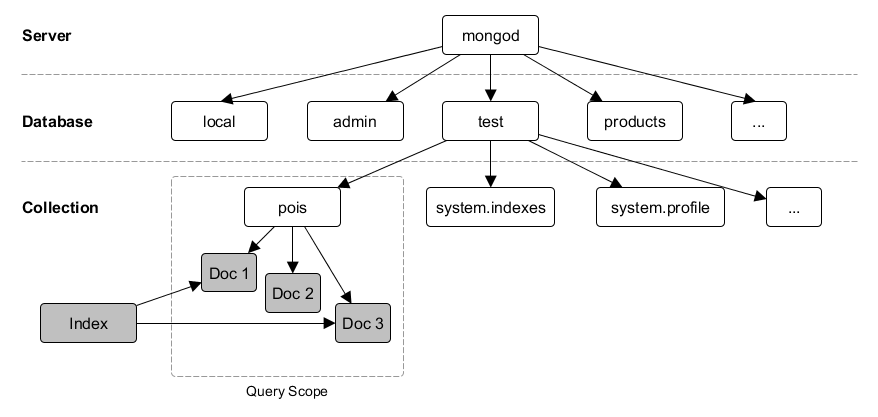
\includegraphics[width=14cm]{images/MongoDB_Architektur.png}
\caption{Graphikdatenbank Beispiel [NoSql 1.9]}
\end{figure}

Letztere Abbildung stellt die grundsätzliche Struktur einer MongoDB-Instanz dar.
Ein \textbf{Server} kann mehrere logische \textbf{Datenbanken} verwalten, die ihrerseits einen oder mehrere logische Namensräume enthalten, die sogenannten \textbf{Collections}. Eine Collection verwaltet die einzelnen Datensätze, die als \textbf{Dokumente} bekannt sind. 
\newline

\textbf{Schema-Freiheit}
\newline
Collections sind schemafrei. Dadurch gibt es für die zugehörigen Dokumente kein vorausgesetztes Schema. Aufgrund der Schema-Freiheut dürfen dennoch Architekturentscheidungen bei der Datenmodellierung nicht ignoriert werden. Stattdessen werden diese Entscheidungen des Schema-Managements auf die Anwendungsentwicklung verlagert.
\newline


\textbf{BSON}
\newline
Während MongoDB für Datenaustausch das JSON-Format nutzt, hält es seine Dokumente im Binary JSON-Format (BSON), einer binärcodiertem Erweiterung des JSON-Formats. Daten im BSON-Format enthalten zusätzlich Informationen zum Typ und zur Länge der Informationen, wodurch schnelleres Parsen von Daten möglich ist. Des Weiteren werden ist BSON um zusätzliche Datentypen wie 32- und 64-bit Integer oder das Datum erweitert. [MongoDb1.8 https://www.mongodb.com/json-and-bson] 
\newline

\begin{lstlisting}
/* JSON */
{"hello": "world"}  // "key":"value"

/* BSON */
\x16\x00\x00\x00           // total document size
\x02                       // 0x02 = type String
hello\x00                  // field name
\x06\x00\x00\x00world\x00  // field value
\x00                       // 0x00 = type EOO ('end of object')
\end{lstlisting}



\textbf{ObjectID und Primärschlüssel}
\newline
Für die eindeutige Identifikation eines Dokuments vergibt MongoDB automatisch erstellte \"\_id\"-Felder. Dabei wird bei der Generierung des BSON-Dokuments für den Wert das \"\_id\"-Feld ein Datentyp "ObjectId" hinzugefügt. Dieses Identifikationsfeld ist gleichzusetzen mit dem Primärschlüsseln aus relationalen Datenbanken. [MongoDB1.85] Ist eine automatische Generierung des eindeutigen Identifikationsfeldes nicht erwünscht, kann der Anwendungsentwickler dieses Feld auch selbst erzeugen, indem er die Eigenschaft explizit dem zu erstellenden Objekt hinzufügt und mit einem Wert verseht. 
\newline


\textbf{Datenbankabfrage}
\newline
Im Vergleich zu relationalen Datenbanken benutzt MongoDB keine Abfragesprache wie SQL. Stattdessen ermöglicht dieses Datenbanksystem drei Arten von Abfragen, wobei eine Abfrage sich immer auf genau eine Collection bezieht. Ein Bezug einer Abfrage zu mehreren Collections, wie es relationale Datenbanken mit „Join“-Operationen erlauben, ist hier nicht gegeben und muss in der Anwendung realisiert werden. [1.9] Abfragen in MongoDB werden grundsätzlich in Form von Dokumenten formuliert. Dieses Verfahren ermöglicht schnelles Abhandeln komplexer Abfragen von tief geschachtelten Dokumentenstrukturen. Nachfolgend werden die drei Abfragemöglichkeiten erläutert.
\newline 
\newline
\textbf{Query-by-Example}
\newline

Das folgende Beispiel zeigt einen Aufruf aller Einträge, die als Ort Karlsruhe eingespeichert haben. 
\newline
\begin{lstlisting}
db.pois.find( {"adresse.ort": "Karlsruhe" } )
\end{lstlisting}

Dabei kommt das Prinzip Query-by-Example [MongoDB2.0] zum Einsatz, bei dem die als JSON-Dokument beschriebenen Suchkriterien als Filter auf die durchsuchte Collection wirkt. Zusätzlich stehen für diese Art von Abfragemöglichkeit sämtliche logische Verknüpfungen und Vergleichsoperatoren zur Verfügung.  [ siehe MongoDB2.1]
Das Ergebnis der obigen Find-Operationen liefert dabei einen Cursor zurück, über den die aufrufende Anwendung durch die einzelnen zurückgelieferten Dokumente iterieren kann. Außerdem kann der Cursor modifiziert werden, um beispielsweise Beschränkungen der Trefferanzahl oder Sortierung vorzunehmen.
\newline
\begin{lstlisting}
db.pois.find().limit(5).sort({"adresse.ort": -1})
\end{lstlisting}


\textbf{MapReduce}
\newline
MapReduce ist ein allgmeines Programmiermodell zur verteilten und parallelen Verarbeitung von großen Datenmengen in aggregierte Ergebnisse. Dabei unterteilt sich der Algorithmus im Wesentlichen in zwei Operationen. [MongoDB2.3]
\newline
-	Map: Emittieren der beliebig vielen Key-Value-Paare für jedes Dokument
\newline
-	Reduce: Zusammenfassen aller Daten, die einem Kriterium entsprechen.
\newline

\textbf{Aggregation-Framework}
\newline
Das Aggregation-Framework bietet als Alternative zum MapReduce-Verfahren den Vorteil der besseren Performance. [MongoDB2.4] Dabei wird eine Pipeline genutzt, die das resultierende Dokument einer Operation an die Eingabe der nächsten Operation weiterleitet. Die entsprechende Funktion ist die Aggregate()-Operation, deren Parameter als Array von Dokumenten die Pipeline-Operatoren abbilden. [MongoDB2.5]
\newline 

\begin{lstlisting}
db.pois.aggregate([
    {$group: {_id: "$adresse.ort", n: {$sum:1}}},
    {$sort: {n: -1}}
])
\end{lstlisting}


Es stehen folgende Pipeline-Operatoren zur Verfügung:

 

\begin{table}[htb]
\begin{center}
    \begin{tabular}{| l | p{14cm} |}
    \hline
    \textbf{Operator}  & \textbf{Beschreibung} \\ \hline
    \$match &Sucht Dokumente analog zu find(). Sollte idealerweise mindesten 1x zu Beginn der Pipeline ausgeführt werden, um die Ergebnismenge einzuschränken.\\
    
    \hline
    \$project & Schränkt auf eine Teilmenge von Feldern ein und verändert die Werte der Felder.  \\
    
    \hline
	\$sort & Sortiert die Dokumente. Analog zu sort() bei find(). .\newline
	Benötigt Private Key und Zertifikat.  \\
	
    \hline    
    \$skip & Überspringt n Dokumente. Analog zu skip() bei find().  \\ 
    
    \hline    
    \$limit &Begrenzt auf n Dokumente. Analog zu limit() bei find().  \\
    \hline 
   \$group   &	Gruppiert nach einem oder mehreren Feldern. \\ 
\$unwind  &	Wird auf ein Array angewendet. Jeder Array-Eintrag generiert dann ein neues Dokument für die nächste Pipeline-Stufe.\\ 
\hline  
\$redact  &	Filtert Felder und Teilbäume des Dokuments in Abhängigkeit vom Inhalte anderer Felder.\\ 
\hline  
\$out  &	Leitet das Ergebnis der Aggregation in eine Collection um. Kann nur als letzter Operator verwendet werden.  \\ 
    
    \hline
    \end{tabular}
\end{center}
\caption{Aggregation Framework: Pipeline-Operatoren [MongoDB1.9]}
\end{table}

\textbf{CRUD}
\newline
MongoDB unterstützt eine Vielzahl an Operationen zum Erzeugen, Lesen, Updaten und Löschen von Daten.
Über folgende Kommandos lassen sich die CRUD-Operationen realisieren:
\newline

\begin{table}[htb]
\begin{center}
    \begin{tabular}{| l | p{8cm} | l |}
    \hline
    \textbf{Operation} & \textbf{Beschreibung} & \textbf{MongoDB Methode} \\
    
    \hline
    Create & Datensätze erstellen & .Insert() \\
    
    \hline
	Read & Datensätze lesen & .Find() \\
	
    \hline    
    Update & Daten aktualisieren & .Update() \\ 
   
    \hline    
    Delete & Datensätze entfernen & .Remove()  \\ 
    
    \hline
    \end{tabular}
\end{center}
\caption{Aggregation Framework: Pipeline-Operatoren [MongoDB1.9]}
\end{table}

\textbf{Create}
\newline
„InsertOne()“ erzeugt ein einzelnes Dokument in der jeweiligen Collection der Datenbank. Dabei wird ein Dokument im JSON-Format als Parameter mitgegeben. ObjectID wird, wenn nicht als Eigenschaft im Dokument angegeben, automatisch von MongoDB erzeugt. Ebenfalls wird die angesprochene Collection automatisch erzeugt, falls sie nicht bereits existiert. Die Funktion „InsertMany()“  erlaubt das Hinzufügen mehrerer Datensätze über ein Array von JSON-Dokumenten als Parameter. Die Methode „Insert“ ist flexibler und bietet beide Parametrisierungsmöglichkeiten. [Mongo2.55 ]
\newline
\begin{lstlisting}
db.personen.insertOne({"vorname" : "Robin"});
\end{lstlisting}

\textbf{Read}
\newline
Um Datensätze aus der Datenbank zu lesen, wird die find()-Methode zur Verfügung gestellt. Sie gibt alle Dokumente einer Kollektion zurück. Wie im Kapitel Query-By-Example beschrieben, kann die Funktion mit Filtern versehen werden. Die Funktion findOne() bietet die gleiche Funktionsweise, die Dokumentenausgabe ist aber auf ein einzelnes Dokument begrenzt.
\newline
\textbf{Update}
\newline
Die Update()-Methode ermöglicht es, Änderungen an Datensätzen vorzunehmen.  Die Methode erhält zwei Parameter, einen zur Angabe der gesuchten Dokumente und den anderen mit  der vorzunehmenden Änderung. Simultan zu den Insert-Methoden gibt es die UpdateOne()-Methode für Änderungen an einem Dokument und UpdateMany()-Methode für mehrere Dokumente.
\newline

\begin{lstlisting}
db.personen.updateOne({"vorname" : "Robin"} , currentDate("last_login") );
\end{lstlisting}

\textbf{Delete}
\newline
Für das Löschen von Datensätzen aus einer Collection gibt es die DeleteOne()- und DeleteMany()-Methode. Über mitgegegeben Parameter können Filter eingestellt werden. Eine ganze Collection kann mit der drop()-Methode entfernt werden.
\newline

\begin{lstlisting}
db.personen.deleteOne( {"vorname" : "Robin"} );
\end{lstlisting}

\textbf{2.2.2.2 Atomare Operationen}
\newline
Als atomare Operationen wird ein Verbund von Einzeloperationen bezeichnet, der als logische Einheit betrachtet wird und nur als Ganzes erfolgreich abläuft oder fehlschlägt. In Bezug auf Datenbanken spricht man von Transaktionen, die entweder als Ganzes erfolgreich ablaufen (Commit) oder nach einer fehlerhaften Einzeloperation rückgangig gemacht werden (Rollback). Ohne atomare Operationen können Probleme aufkommen, die zu einer Inkonsistenz der Datenzustände führt. Beispielsweise wurde ein Abbruch inmitten mehrerer zusammenhängender Operationsabläufe dazu führen,  dass nur ein Teil der Operationen ausgeführt wurde, während die restlichen Operationen und somit die verbleibenden Datenänderungen verworfen werden.
\newline
Bis vor dem Jahre 2018 unterstützte MongoDB keine Transaktionen. Mit der Veröffentlichung der Version 4.0 wurde der Funktionsumfang von MongoDB stark erweitert. Eines der neuen Erweiterungen war die Möglichkeit, Transaktionen durchführen zu können. Dafür werden sogenannte „Sessions“ genutzt. Sämtlichen CRUD-Operationen, die einer Transaktion zugehören sollen, werden eine Session als zusätzlicher Parameter hinzugefügt.  Bei Abschluss der Transaktion kann sie mit der Methode „session.commitTransaction()“ bestätigt werden. Andernfalls, sollte ein Fehler aufgetreten sein, kann die Methode „session.abortTransaction()“ die Operationen rückgängig machen. Eine wichtige Vorraussetzung, um Transaktionen in MongoDB nutzen zu können, ist ein Replica Set aufzusetzen. Darauf wird im weiteren Kapitel eingegangen. 
\newline

\textbf{2.2.4.x Architektur}
\newline 
Wired Tiger?
Storage Engine
Replica Sets
Oplog
Sharding
\newline

\textbf{Technische Grundlagen}
/
Replica
Transaktionen
\newline

\textbf{Verwaltungswerkzeuge}
Mongo Shell
Treiber
Grafische Oberflächen
